本章简要介绍本文后续方案中涉及的基本概念和技术。主要包含有无人机的基本飞行控制逻辑和其安全相关模块,方案中使用的机器学习与模糊测试相关的内容。

\section{无人机飞行控制与模块}
无人机飞行控制简称飞控,可以看作飞行器的大脑。
多轴飞行器的飞行、悬停,姿态变化等等都是由多种传感器将飞行器本身的姿态数据传回飞控,再由飞控通过运算和判断下达指令,由执行机构完成动作和飞行姿态调整。
无人机的硬件和软件是紧密相连的,其核心是飞行控制程序,其功能主要是解析任务和飞行状态,包选择合理的飞行速度,处理传感器的回传速度。
从抽象的角度看,无人机的控制系统主要分为以下几个模块。

\begin{itemize}
\item \textbf{飞行控制器}:飞行控制器是无人机的大脑,负责处理传感器数据、执行飞行算法并控制无人机的姿态和运动。常见的飞行控制器包括Pixhawk、DJI Naza等。

\item \textbf{飞行控制软件}:如\tool{Ardupilot}~\cite{ardupilot} 和 \tool{PX4}~\cite{px4},
  它提供高级功能以实现复杂的飞行模式,包括无人机的自动驾驶,特殊飞行动作,飞行中的障碍规避,飞行异常处理等。

\item \textbf{姿态传感器}:姿态传感器用于测量无人机的姿态,包括加速度计、陀螺仪和磁力计。这些传感器提供了关于无人机当前方向、倾斜和旋转的数据。

\item \textbf{遥控器}:遥控器是飞行员用来操控无人机的设备,通过遥控器飞行员可以控制无人机的飞行姿态、速度和航向。

\item \textbf{遥控接收器}:遥控接收器接收遥控器发送的指令,并将这些指令传递给飞行控制器,以控制无人机的飞行。

\item \textbf{电调}:电调控制无人机的电机转速,根据飞行控制器发送的指令调整电机的转速,从而控制无人机的姿态和飞行。

\item \textbf{GPS模块}:GPS模块用于定位无人机的位置,提供全球定位系统数据,帮助无人机进行定点悬停、航线飞行和返航等功能。

\item \textbf{通信模块}:通信模块用于无人机与地面站或其他设备之间的通信,传输飞行数据、视频信号和遥控指令。

\end{itemize}


% \begin{itemize}
%   \item \textbf{飞行控制软件:}(如\tool{Ardupilot}~\cite{ardupilot} 和 \tool{PX4}~\cite{px4}),
%   它提供高级功能以实现复杂的飞行模式,包括无人机的自动驾驶,特殊飞行动作,飞行中的障碍规避,飞行异常处理等。
%   \item \textbf{控制器硬件:} (如\tool{Pixhawk}、\tool{Bebop}和\tool{Navio2},作为飞行控制和数据处理的基本平台,为飞行控制软件提供算力基础。
%   为各种传感器的数据汇总通过一个集束平台。
%   \item \textbf{低级硬件:} 无人机的数据和动力来源,系统使用一些传感器(如气压计、陀螺仪、加速计、磁力计和GPS)进行导航和感知。原始传感器数据捕捉到车辆在环境中的物理状态(例如,角度和线性位置),并帮助计算执行器信号(例如,转子速度、转向),以便将车辆定位到下一个状态。将车辆定位到下一个状态。
%   此外,无人机程序一般还提供其他高级功能以便使用者可以应用到各个飞行场景。以及提供各种安全保障机制。
%   以及飞行所需的动力来源,电机。由控制软件直接下达相应的转速以实现规定的飞行姿态。
% \end{itemize}

\subsection{无人机飞行控制}\label{moti:pre_study}
% 需要说明飞行控制算法的核心,GPT生成?
无人机机身是由对称的十字形刚体结构构成,在十字形结构的四个端点分别安装一个由两片桨叶组成的旋翼为飞行器提供飞行动力,每个旋翼均安装在一个电机转子上,通过控制电机的转动状态控制每个旋翼的转速,来提供不同的升力以实现各种姿态。
对于一个给定的飞行路径,无人机通过一系列高层次的状态转换,将任务转换成电机应有的转速以驱动飞行。
图~\ref{fig:rawcontrol}展示了该程序的控制过程。

给定一个命令,飞行控制程序根据之前的状态、当前的状态、传感器感知数据(如来自GPS、陀螺仪和加速度计)和飞行配置,预测下一个期望状态(即\emph{参考状态})。
大多数无人机利用多传感器测量来获得对物理状态的更准确视图,因为单个传感器在真实环境中无法提供可靠数据(由于传感器噪声、可能的传感器故障等)。
在四旋翼飞行器中,多个冗余或异构传感器(例如陀螺仪、加速度计和GPS)使控制器能够识别当前物理状态和环境,然后相应地控传感器融合不局限于相同类型的传感器。
复杂的传感器融合算法(例如扩展卡尔曼滤波器)通常利用异构传感器数据来减少不确定性并产生更准确的测量。
随后,控制算法更具具体的测量结果并结合任务目标,产生执行器信号(例如,电机指令)来驱动无人机达到参考状态。


\begin{figure}[ht]
  \centering
    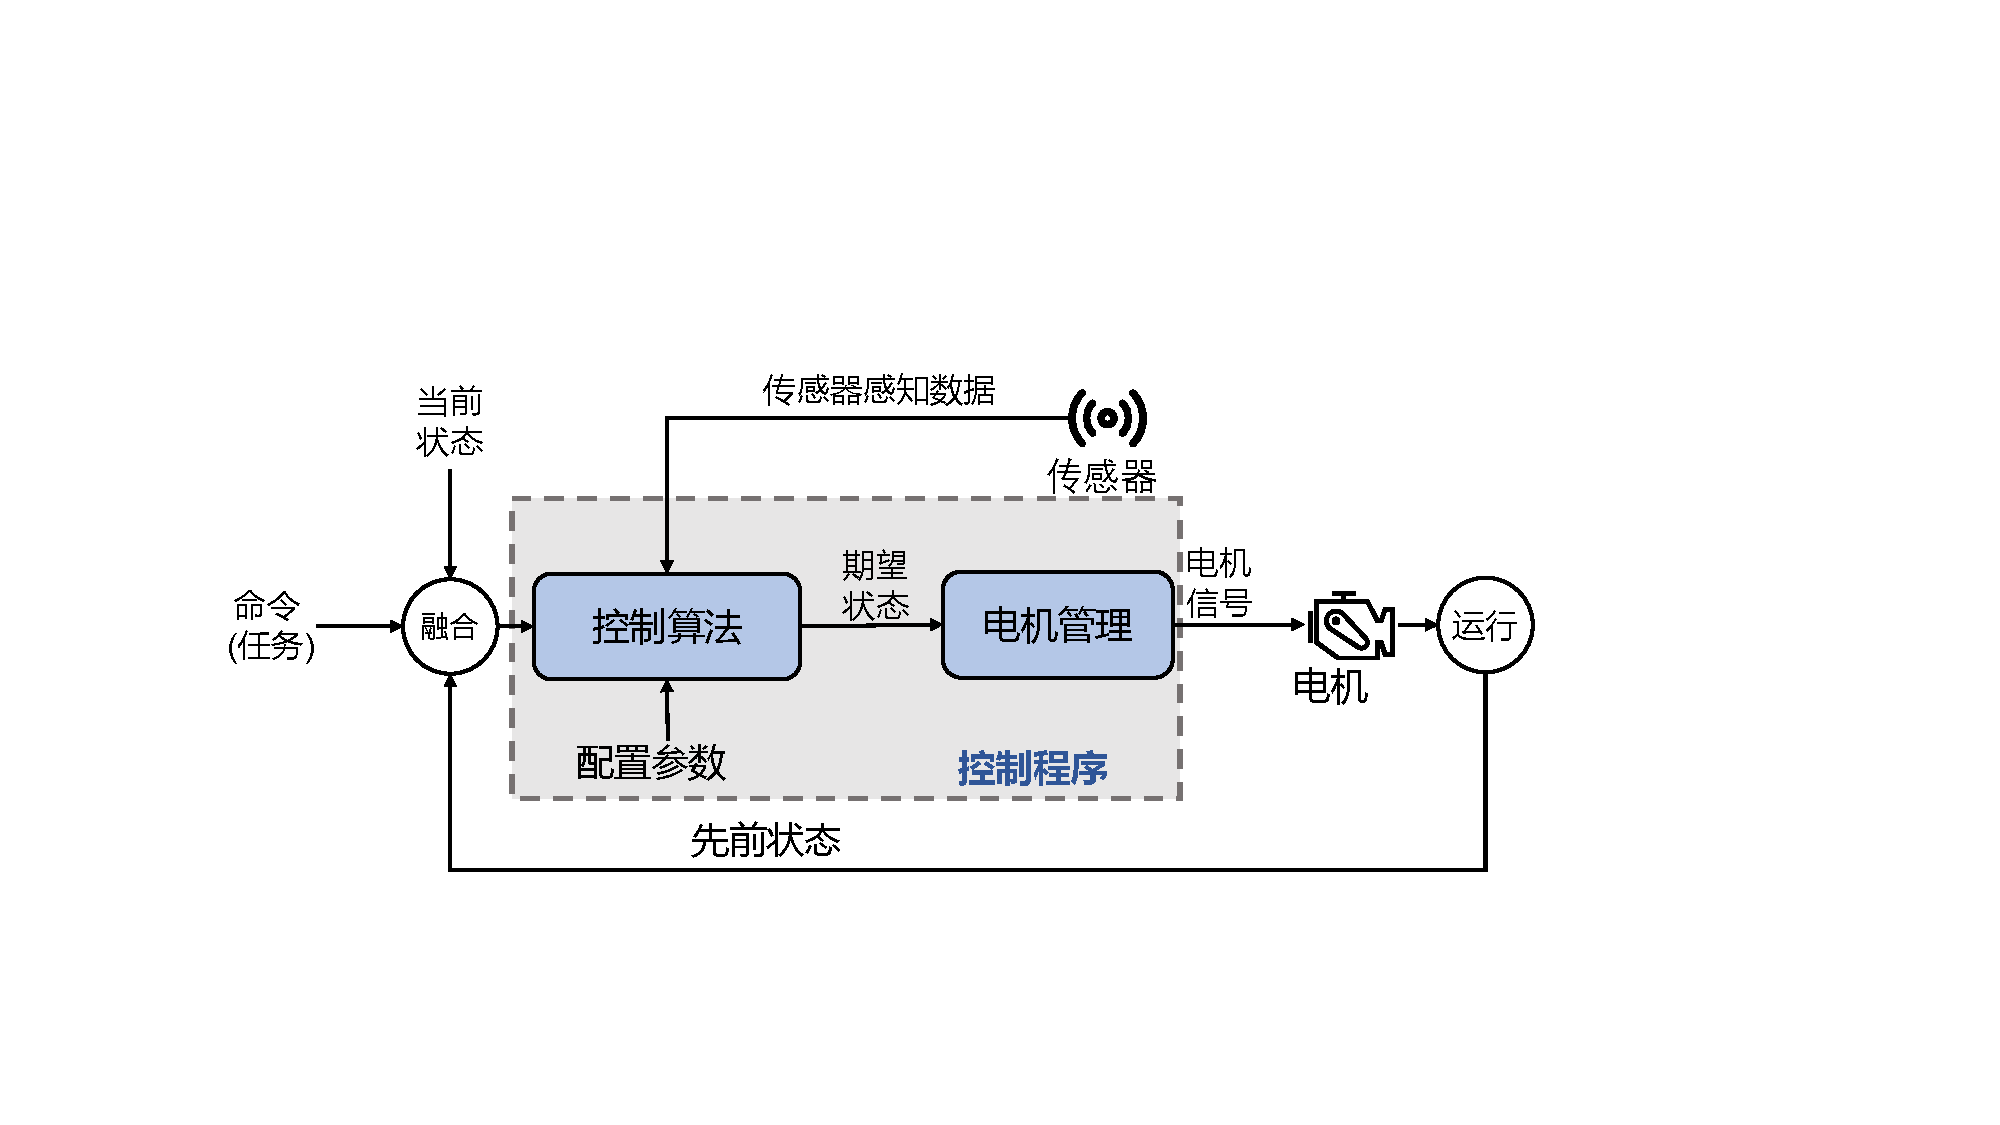
\includegraphics[width=\columnwidth]{fig/background/rawcontrol.pdf}
\caption{无人机飞行控制程序的控制逻辑}
\label{fig:rawcontrol} 
\end{figure}

% 说明存在飞行偏差这一个事实,无人机也是根据这个进行调整的。
然而,真实状态和参考状态并不总是匹配。
如果实际飞行状态和参考状态之间的偏差很小,所以电机可以纠正它,那么飞行状态被认为是稳定的。
否则,飞行状态就被认为是不稳定的。
尽管一些不稳定的状态可以通过发送特定的指令来纠正,但如果偏差累积起来,超过了电机的纠正能力,无人机就会变得不可控。
最终,飞行任务将不得不中断。
图~\ref{fig:des&ach}显示了无人机滚动角度的姿态变化导致了一个不稳定的飞行(红色区域)。
其中实线表示控制器所期望的程度。
虚线表示无人机实际完成的角度,以及底部的直方图(棕色条)表示这两条曲线之间的误差。
从图中可以清楚得观察到,期望的角度和实现的角度在开始时差别不大,但随后增加,导致飞行不稳定。

\begin{figure}[ht]
  \centering
    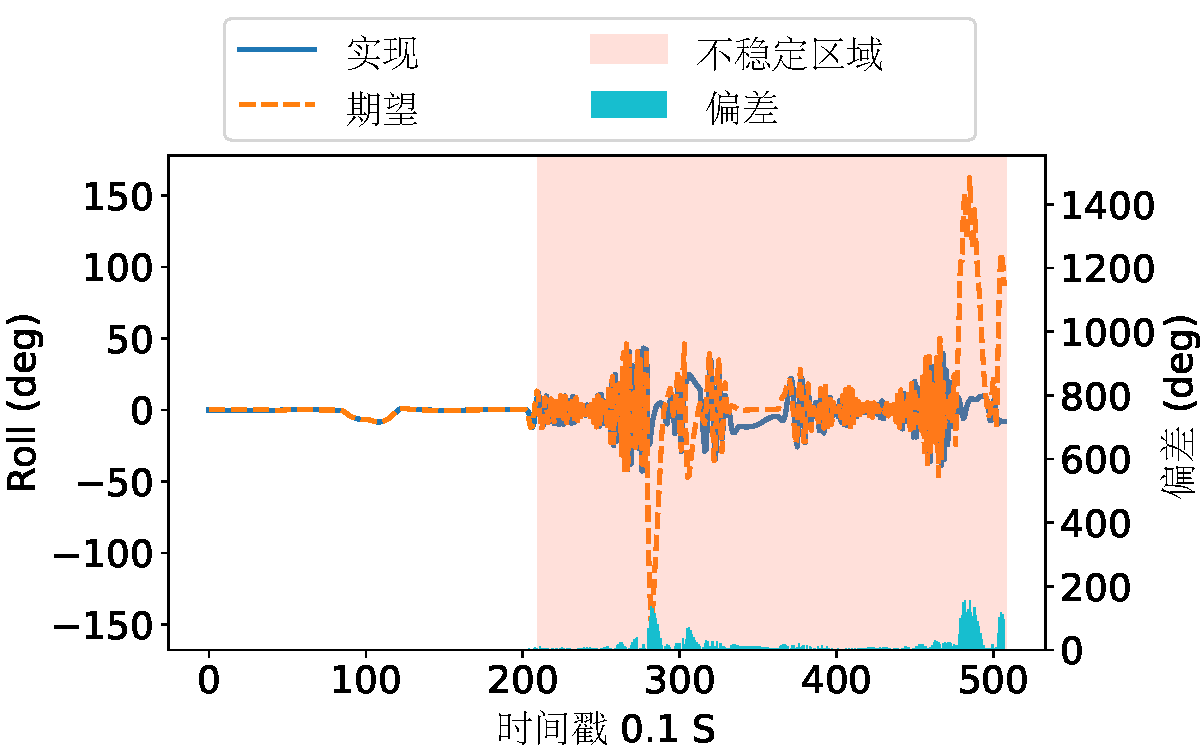
\includegraphics[width=0.9\columnwidth]{fig/background/des&ach.pdf}
\caption{飞行中Roll角的变化.}
\label{fig:des&ach} 
\end{figure}


\subsection{无人机参数控制}\label{subsec:drone_control}
制造商提供由数百个参数组成的可配置控制方案,以支持各种飞行任务。
每个用户/控制台可以通过调整这些参数值来控制无人机,以应对不同的任务场景。
无人机的调试工作很大一部分是对飞行控制参数的调试,广义的飞控参数包含了制导、导航、控制律以及各种控制策略中的可调参数。
一般的飞控都有上百项需要人为调试的参数,有的甚至是几百上千个。而姿态控制作为无人机控制的基础
同时为了保证人员在调试时的安全设定,制造商提供了一种范围控制机制,通过每个参数的预设值范围指导参数选择。

以常用的飞行控制程序\tool{Ardupilot}为例。
代码~\ref{lis:range_bug_code_example} 片断展示了了其飞行控制程序中如何使用参数,\param{PSC\_VELXY\_P},来控制飞行。
在变量声明之后(第6行),\param{PSC\_VELXY\_P}(代码中的\param{k\_param\_pi\_vel\_xy})被分配到一个控制值(第3行)。
飞行控制程序应用这个值来转换角度控制器的增益(第10行至第12行)。
该程序片段同时会校验当前设置的参数值是否会超出了官方预先设定的范围。
通过这种调整机制,无人机的飞行控制程序可以通过更改配置参数从而适应不同的无人机类型,飞行环境和任务需要。
\begin{listing}[ht]
\scriptsize{
\begin{minted}[linenos, firstnumber=8,breaklines,xleftmargin=2em,numbers=left]{c++}
//"PSC_VELXY_P", 0.1, 6;
...
ConversionInfo angle_and_filt_conversion_info[] = {
...
 // PARAMETER_CONVERSION - Added: Jan-2018
{ Parameters::k_param_pi_vel_xy, 0, AP_PARAM_FLOAT, "PSC_VELXY_P" },
}
...
// convert angle controller gain and filter without scaling
for (const auto &info : angle_and_filt_conversion_info) {
    AP_Param::convert_old_parameter(&info, 1.0f);
}
\end{minted}
}
\caption{参数\param{PSC\_VELXY\_P}使用的代码样例}
\label{lis:range_bug_code_example}
\end{listing}


\subsection{无人机安全检查}
% 安全检查
为了减轻潜在的不安全后果,开发者为控制程序设计了各种安全检查机制,以检测异常情况,同时提供反补救措施。
通过应用来自传感器和状态估计的内部无人机信息,这些检查设计了触发条件,以检测特定的突发情况(如崩溃、推力损失)。
当这些条件得到满足时,系统将提出安全警告并启动相应的补救措施。
开发人员通常使用他们的领域知识和经验来构建条件规则。

例如,以 \tool{ArduPilot}为例。
表~\ref{tab:condition}展示了\tool{ArduPilot}工具中的两个安全检查模块及其触发条件。
\emph{崩溃}和\emph{推力损失}。
\emph{碰撞}模块在车辆可能失去控制并撞上物体的情况下解除电机,这可以减少对车辆的损害和对车辆附近的人的伤害。
它在系统中验证四个内部数值,以判断当前飞行不安全:无人机的加速度小于$3m/s$,倾斜角大于$15$度,系统计算的角度误差大于$30$度,无人机速度小于$10m/s$。
\emph{推力损失}模块旨在检测推进系统的硬件故障,即无人机无法再达到要求的姿态和油门输出,因为一个或多个电机在$100\%$的油门下饱和。
如果这种情况持续了很长时间,姿态控制可能无法保持稳定。
该模块验证四个值:控制程序的期望角度大于$15$度,沿$Z$轴的速度为负值,系统计算的角度误差大于$30$度,其油门变得饱和。

\begin{table}[ht]
\caption{Ardupilot官方源代码中的崩溃和推力损失触发条件}
\label{tab:condition}
\centering
\begin{tabular}{c|c|c}
        \toprule[1.5pt]
        \textbf{检查模块} & \multicolumn{2}{c}{\textbf{触发条件}} \\
        \midrule[0.8pt]
        \multirow{2}{*}{崩溃} & 加速度 $ < 3m/s$  &  倾斜角 $ > 15 deg$ \\
        \cmidrule[0.8pt]{2-3}
          & 角度错误 $ > 30 deg$  &  加速度 $ < 10m/s$  \\
        \midrule[0.8pt]
        \multirow{2}{*}{动力损失} & 期望角 $ > 15 deg$  &  Z轴速度为负 \\
        \cmidrule[0.8pt]{2-3}
          & 角度错误 $ > 30 度$  &  油门饱和  \\
        \bottomrule[1.5pt]
\end{tabular}
\end{table}


\section{时间序列预测}
% LSTM和TCN的模型介绍
时间序列预测是一种利用历史和当前数据来预测一段时间内或未来特定时间点的未来值的技术。 
通过分析过去存储的数据,可以做出明智的决策,这些决策可以帮助了解未来趋势。
在机器学习问题中,时间序列的预测被转化为监督学习问题。
算法利用窗口滑动,从时间序列中连续取样,作为生成不同的输入和输出。
下面将介绍两种本文涉及的时间序列预测方法。

\subsection{长短期记忆网络}
长短期记忆网络(Long Short Term Memory,LSTM)~\cite{hochreiter1997long},即长短期记忆网络,一种循环神经网络(Recurrent Neural Network,RNN)~\cite{rnn}的变体。
LSTM专门用于处理有前后关联性的序列数据,具有记忆和长期依赖建模的能力。
LSTM通过添加成为\dquote{门}的结构来控制相关信息的流动,从而解决了传统RNN中存在的梯度消失和梯度爆炸问题,使其能够更好地捕捉长期依赖关系。

LSTM的核心思想是三种不同的\dquote{门}单元,分别为输入门(Input Gate)、遗忘门(Forget Gate)、输出门(Output Gate)。
这些门控单元通过学习的方式来决定是否允许信息通过,从而控制信息在网络中的流动。
其中,输入门决定了当前时刻输入的信息有哪些需要被保留下来,它通过一个激活函数来生成一个0到1之间的值,表示这个信息的权重,也就是信息的重要性。
这个重要性值与输入经过一个tanh激活函数后的值相乘,得到了当前时刻的记忆候选值。
遗忘门决定了前一时刻有哪些信息和记忆要被遗忘。
它使用一个sigmoid激活函数同样生成一个0到1之间的值,表示前一时刻记忆二点重要性。
同样得,这个重要性值与前一时刻的记忆相乘,得到了被保留的记忆。
然后,输出门决定了当前时刻的输出有多少要被传递出去。
它也包含一个sigmoid激活函用于评判输出的重要性,然后与一个tanh激活函数后的值相乘,得到了当前时刻的输出。
最终,LSTM使用当前时刻的输入、前一时刻的记忆和门控单元的输出来更新当前时刻的记忆。
这个更新过程包括遗忘门决定的前一时刻记忆的遗忘部分,输入门决定的当前时刻输入的记忆部分,以及门控单元的输出。
通过这种门控机制,LSTM能够有效地保留和遗忘信息,从而更好地处理长期依赖关系。
它在处理序列变化数据方面比普通的神经网络更好。
诸如高维度、分散性和高噪音等问题。噪声存在的问题,这些问题是传统算法无法处理的问题。

下面将以公式化的方式进行说明。
假设在时间戳$t$,输入为$x_t$,上一时刻的隐藏状态为$h_{t-1}$,上一时刻的细胞状态为$c_{t-1}$,当前时刻的隐藏状态为$h_t$,当前时刻的细胞状态为$c_t$。
LSTM的计算过程可以分为三个门和一个记忆单元,分别为遗忘门、输入门、输出门和细胞状态更新:
\begin{itemize}
    \item \textbf{遗忘门(Forget Gate):}
遗忘门决定哪些信息需要从细胞状态中丢弃。遗忘门的计算公式如下:
\begin{equation}
    f_t = \sigma(W_f \cdot [h_{t-1}, x_t] + b_f)
\end{equation}

\item \textbf{输入门(Input Gate):}
输入门决定哪些新信息需要存储到细胞状态中。输入门的计算公式如下:
\begin{equation}
    i_t = \sigma(W_i \cdot [h_{t-1}, x_t] + b_i)
\end{equation}
\begin{equation}
    \tilde{c}_t = \tanh(W_c \cdot [h{t-1}, x_t] + b_c)
\end{equation}

\item \textbf{更新细胞状态:}
使用遗忘门和输入门的信息来更新细胞状态。更新细胞状态的计算公式如下:
\begin{equation}
    c_t = f_t \odot c_{t-1} + i_t \odot \tilde{c}_t
\end{equation}

\item \textbf{输出门(Output Gate):}
输出门决定当前时刻的隐藏状态$h_t$。输出门的计算公式如下:
\begin{equation}
    o_t = \sigma(W_o \cdot [h_{t-1}, x_t] + b_o)
\end{equation}
\begin{equation}
    h_t = o_t \odot \tanh(c_t)
\end{equation}

\end{itemize}

其中,$(W_f, W_i, W_c, W_o)$ 是权重矩阵,$(b_f, b_i, b_c, b_o)$ 是偏置向量,$([h_{t-1}, x_t])$ 表示将隐藏状态和输入连接起来,$\sigma$ 是sigmoid函数,$\odot$ 表示逐元素相乘操作,$\tanh$ 是双曲正切函数。




\subsection{时间卷积网络}
时间卷积网络(Temporal Convolutional Networks,TCN) ~\cite{bai2018empirical},是一种用于处理序列数据的深度学习模型,他的核心架构是基于卷积神经网络的(Convolutional Neural Network,CNN)~\cite{schmidhuber2015deep}。
TCN能够有效地捕捉序列数据中的长期依赖关系。
与传统的循环神经网络相比,TCN的主要优势在于并行计算的能力和对长期依赖的建模能力。
传统的RNN在处理长序列时容易出现梯度消失或梯度爆炸的问题,而TCN通过使用一维卷积层来捕捉不同时间步之间的依赖关系,避免了这些问题的出现。
此外,TCN还可以并行计算,加速了模型的训练和推断过程。
TCN的核心思想是通过一维卷积层来进行特征提取和建模。
该卷积层可以捕捉局部的时间相关性,并通过多个卷积层堆叠来扩展对于序列中信息的感受视野,从而捕捉更长期的依赖关系。
为了解决卷积层的输出长度问题,TCN引入了残差连接(Residual Connections)~\cite{he2016deep}和空洞卷积(Dilated Convolutions)~\cite{yu2015multi}的技术。
残差连接可以保留原始输入的信息,避免信息的丢失和模型的退化。而空洞卷积则通过增大卷积核的感受野,使得卷积层能够同时捕捉不同时间尺度的依赖关系。
这种方法使CNN非常深,但由于大规模并行处理的优势,它可以被并行处理,无论网络有多深,都可以节省大量的时间。

假设在时间步$t$,输入为$x_t$,TCN的核心是通过卷积操作来捕捉时间序列数据中的长期依赖关系。
TCN的计算过程的公式化描述如下:
\begin{itemize}
    \item \textbf{卷积操作:} TCN使用多层卷积层来提取时间序列数据的特征。
    假设第$l$层卷积层的输入为$z(l-1)$,输出为$z(l)$,卷积核为$w(l)$,偏置为$b(l)$,卷积操作可以表示为:
    \begin{equation}
        z_t(l) = \sigma(w(l) \ast z_{t-k}(l-1) + b(l))
    \end{equation}
    其中$\ast$表示卷积操作,$\sigma$是激活函数,$k$是卷积核的大小。

    \item \textbf{残差连接:}为了加快训练速度和提高模型性能,TCN通常采用残差连接。
    \begin{equation}
        z_t(l) = z_t(l-1) + z_t(l)
    \end{equation}

    \item  \textbf{池化操作:} 池化操作有助于减少特征的维度,提取最重要的特征。常用的池化操作包括最大池化和平均池化。
    最大池化的计算公式如下:
    \begin{equation}
        z_t(l) = \max(z_{t-j}(l))
    \end{equation}
    其中$j$是池化窗口的大小。

    \item \textbf{输出层:} 最后一层卷积层的输出可以通过全连接层或者其他适当的操作来得到最终的输出。假设最后一层卷积层的输出为$z(l)$,输出层的计算可以表示为:
    \begin{equation}
        y_t = \text{softmax}(W_{\text{out}} \cdot z_t(l) + b_{\text{out}})
    \end{equation}
    其中$W_{\text{out}}$是输出层的权重矩阵,$b_{\text{out}}$是输出层的偏置向量 。
\end{itemize}


\section{不变量验证}
不变量的字面是表达\dquote{不会改变的量}。
它是一种重要的数学和物理方法,用于检验系统在不同条件下是否遵守某些基本规律或性质。
在数学和物理学中,不变量是指在系统变化过程中保持不变的物理量或性质。
在工程学中,不变量验证通常用于检验工程模型的稳定性和准确性。
在现实世界的应用中,这种不变量是由开发者手动分配的,或者由程序分析自动生成。
例如,在有限元分析中,工程师可以利用不变量验证来确保模型在不同网格密度下的数值解是否收敛到正确的结果。
通过验证一些数学量(如误差估计、残差等)的不变性,工程师可以评估模型的准确性和可靠性。
除非发生模式偏差或外部影响,否则对象的变量应始终遵循不变性约束。

同时也是不变量的这一特性,如果对象约束出现明显偏离于不变量约束的模式,则会被认为是出现了异常。
例如,DAIKON~\cite{ernst2001dynamically}提取一个明确的程序不变式,在修改代码时可以保留程序属性,并利用它来检测运行时异常。
运行时验证~\cite{rocsu2009runtime}利用flow invariant,通过检查控制流来验证合法的程序状态转换。
S3FD~\cite{zhang2017s3fd}提出了一个基于尺度的不变性,以实现实时人脸检测,而不考虑相机距离。
Choi~\cite{choi2018detecting}设计了一个机器人车辆的控制不变性,以监测异常控制数据来提出攻击警告。
这些研究表明,不变性检查可以描述广泛的面向软件(即网络)的异常情况。


\section{遗传算法模糊测试}
遗传模糊测试(Genetic Fuzzing)是一种结合遗传算法(Genetic Algorithm,GA)和模糊测试(Fuzzing)的测试技术,用于发现软件系统中的漏洞和错误。
它通过自动化地生成、变异和评估输入数据,以探索软件中存在的异常行为,且可以是动态的或者静态的。
遗传算法是一种启发式优化算法,模拟了生物进化的过程。
自然界生物在周而复始的繁衍中,基因的重组、变异等,使其不断具有新的性状,以适应复杂多变的环境,从而实现进化。
遗传算法精简了这种复杂的过程而抽象出一套数学模型,用较为简单的编码方式来表现复杂的现象,并通过简化的遗传过程来实现对复杂搜索空间的启发式搜。
它通过使用基因表示解空间中的候选解,并利用选择、交叉和变异等操作来搜索最优解。
在遗传模糊测试中,遗传算法被用于生成和演化输入数据,以尽可能地覆盖软件系统的不同执行路径。
而将遗传算法与模糊测试相结合,可以对模糊测试的目标进行全局寻优,提高模糊测试的覆盖准确度,降低无效测试的概率。
遗传模糊测试的流程通常包括以下几个步骤:

\begin{itemize}
  \item \textbf{初始化种群:} 初始时,随机生成一组输入数据,称为种群。每个输入数据都被视为一个个体,具有一定的基因表达。
  \item \textbf{评估适应度:} 将种群中的每个个体输入到待测试的系统中,并评估其执行结果。适应度函数用于评价个体在测试中的表现,通常是基于代码覆盖率、错误率或其他测试目标。
  \item \textbf{选择操作:} 根据个体的适应度,在种群中选择一部分个体作为父代,用于下一代的繁殖过程。通常采用轮盘赌选择或排名选择等策略。
  \item \textbf{交叉操作:} 从选定的父代中,随机选择两个个体,并通过交叉操作生成新的个体。交叉操作模拟了生物遗传中的基因交换过程,以产生更多的遗传变异。
  \item \textbf{变异操作:} 对新生成的个体进行变异操作,以引入更多的随机性和多样性。变异操作模拟了生物遗传中的基因突。
  \item \textbf{更新种群:} 将生成的新个体加入到种群中,并删除一部分适应度较低的个体,以保持种群的规模稳定。
  \item \textbf{迭代终止:} 根据预设的终止条件(例如达到最大迭代次数或满足特定的测试目标),决定是否终止遗传模糊测试的过程。
\end{itemize}

\section{深度确定性策略梯度DDPG}
强化学习(Reinforcement Learning,RL)是一种机器学习方法,旨在通过智能体(Agent)与环境的交互学习如何做出最优决策。
在强化学习中,智能体通过观察环境的状态,采取动作,并获得奖励分数来学习如何在不同状态下做出最优的决策策略。
强化学习的目标是通过与环境的交互,使智能体学会最大化累积奖励的策略。

深度强化学习策略(Deep Deterministic Policy Gradient,DDPG)~\cite{lillicrap2015continuous}是一种基于深度学习的强化学习算法,专门用于解决连续动作空间的问题。
DDPG算法的核心思想是使用深度神经网络来近似值函数和策略函数。它包含两个主要的网络:一个是Actor网络,用于学习策略函数,根据当前状态输出一个动作;
另一个是Critic网络,用于学习值函数,根据当前状态和动作输出一个值函数估计。
DDPG算法通过不断地在经验回放缓冲区中采样并更新这两个网络,来优化策略和值函数的参数。

DDPG算法的步骤如下:
\begin{itemize}
  \item \textbf{初始化:} 初始化Actor网络和Critic网络的参数。
  \item \textbf{环境交互:} 根据当前状态使用Actor网络选择一个动作。
  执行选择的动作并观察环境反馈的下一个状态和奖励。
  将状态、动作、奖励和下一个状态存储到经验回放缓冲区中。
  从经验回放缓冲区中随机采样一批数据。
  \item \textbf{更新Critic网络的参数:} 根据下一个状态和Actor网络的目标动作,使用Critic网络计算目标Q值。
  使用Critic网络计算当前状态和动作的Q值。
  使用目标Q值和当前Q值之间的均方差作为损失函数。
  通过梯度下降法最小化损失函数来更新Critic网络的参数。
  \item \textbf{更新Actor网络的参数:} 根据Critic网络的输出和Actor网络的动作,计算Actor网络的策略梯度。
  通过梯度上升法最大化策略梯度来更新Actor网络的参数。
  \item \textbf{条件停止:} 重复上述步骤,直到达到预设的停止条件
\end{itemize}

DDPG算法通过不断地在经验回放缓冲区中采样和更新网络参数,逐渐优化策略和值函数,从而学习到在连续动作空间中最优的策略。
